\documentclass[sigconf,nonacm,screen,pbalance]{acmart}
\usepackage{enumitem}
\begin{document}
\title{The Design of Search User Interfaces}
\author{Marti Hearst}
\maketitle

% \section*{Chapter Contents}
% \begin{enumerate}[label={\arabic*.}]
%     \item Keeping the Interface Simple
%     \item A Historical Shift in Search Interface Design
%     \item The Process of Search Interface Design
%     \item Design Guidelines for Search Interfaces
%     \item Offer Efficient and Informative Feedback
%     \item Balance User Control with Automated Actions
%     \item Reduce Short-Term Memory Load
%     \item Provide Shortcuts
%     \item Reduce Errors
%     \item Recognize the Importance of Small Details
%     \item Recognize the Importance of Aesthetics in Design
%     \item Conclusions
% \end{enumerate}
\setcounter{tocdepth}{1}
\renewcommand*\contentsname{Chapter Content}
\tableofcontents
\vspace{-20pt}

\begin{figure}[ht]
    % \vspace{-10pt}
    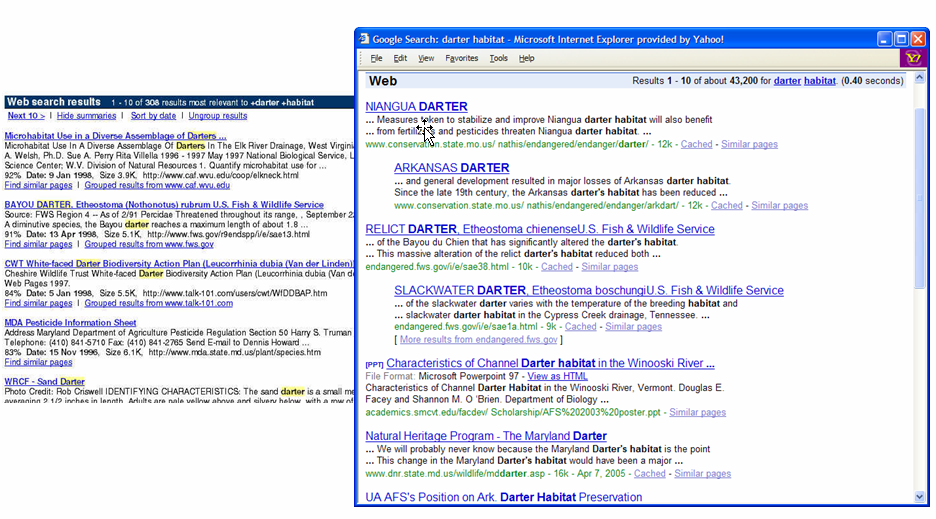
\includegraphics[width=\columnwidth]{./infoseek_vs_google.png}
    \vspace{-20pt}
    \caption{Search results listings from Infoseek in 1997 (left) and Google in 2007 (right), courtesy Jan Pedersen.}
    \label{fig:figure-1}
    \vspace{-10pt}
\end{figure}

\section{Keeping the Interface Simple}

The job of the search user interface is to aid users in the expression of their information needs, in the
formulation of their queries, in the understanding of their search results, and in keeping track of the
progress of their information seeking efforts.

However, the typical search interface today is of the form: type-keywords-in-entry-form,
view-results-in-a-vertical-list. A comparison of a search results page from Google in 2007 to that of
Infoseek in 1997 shows that they are nearly identical (see \autoref{fig:figure-1}). Why is the
standard interface so simple? Some important reasons for the relative simplicity and unchanging nature of
the standard Web search interface are:

\begin{itemize}[leftmargin=1.5em,labelwidth=*]
    \item Search is a means towards some other end, rather than a goal in itself. When a person is looking for
    information, they are usually engaged in some larger task, and do not want their flow of thought
    interrupted by an intrusive interface.

\item Related to the first point, search is a mentally intensive task. When a person reads text, they are
    focused on that task; it is not possible to read and to think about something else at the same time.
    Thus, the fewer distractions while reading, the more usable the interface.

\item Since nearly everyone who uses the Web uses search, the interface design must be understandable and
    appealing to a wide variety of users of all ages, cultures and backgrounds, applied to an enormous
    variety of information needs. 
\end{itemize}

Designers of Web search interfaces have learned that in order to be able to successfully serve their
highly diverse user base, they must be very careful about any complexity that they introduce. Almost any
feature that a designer might think is intuitive and obvious is likely to be mystifying to a significant
proportion of Web users.

To illustrate this point, despite the simplicity of the search results listings shown above, research
suggests that even this spartan presentation is too complex for some people. A study of elderly users by
\href{https://searchuserinterfaces.com/book/sui_references.html#aula2005lim}{Aula and Käki, 2005} found that further simplifying the list of
results reduced errors substantially. And research by \href{https://searchuserinterfaces.com/book/sui_references.html#hargittai2004cac}{Hargittai, 2004} showed that some people do
not understand even the very basics of keyword specification. Unlike most studies that involve
university-educated participants exclusively, Hargittai obtained a random sample of 100 participants
representative of the population of a county in New Jersey according to socio-economic factors. \href{https://searchuserinterfaces.com/book/sui_references.html#hargittai2004cac}{Hargittai, 2004} found that, in addition to
not really understanding keyword queries, many participants confused the address bar with the search entry
form, and vice versa (the latter effect is common, as can be inferred from the fact that the most frequent
queries for all search engines are {\bf  google} and {\bf  yahoo}). Some participants confused the
syntax of the address bar with the syntax of query terms, placing spaces within URLs in the address form,
as in {\bf  www.new york times.com} and {\bf  time warner.com}, or omitting all spaces from their
keywords, resulting in queries like {\bf  presidentalcampaign2000}, {\bf  employmentopportunities}, and
{\bf  fordescort}.

Another study by \href{https://searchuserinterfaces.com/book/sui_references.html#muramatsu2001tqi}{Muramatsu and Pratt, 2001} with 14 participants found that most people had strong misconceptions
about simple Boolean operations. When comparing search engines that automatically applied AND versus OR to
query terms, some assumed the ANDing search engine indexed a smaller collection; most had no explanation
at all. When receiving empty results for the query {\bf  to be or not to be}, two thirds could not
explain this phenomenon in a way that remotely resembled stopword removal. For term order variation in
queries (for example, {\bf  boat fire} vs. {\bf  fire boat}), two thirds did not expect the results to
differ.

Although today's standard search is a big improvement in usability over older command-line based Boolean
systems, there is evidence that keyword querying is not initially intuitive. In fact, the literature
suggests that people who are new to using search engines tend to start by asking a natural language question
(\href{https://searchuserinterfaces.com/book/sui_references.html#bilal2000c}{Bilal, 2000}, \href{https://searchuserinterfaces.com/book/sui_references.html#schacter1998csi}{ Schacter et~al., 1998}). Novice searchers must {\em  learn} to expect that a query
will not yield immediately usable results, and that they must scan search results lists, navigate through
Web sites and read through Web pages to try to find the information they seek. A study by \href{https://searchuserinterfaces.com/book/sui_references.html#pollock1997swi}{Pollock and Hockley, 1997} found that, for novice searchers, the notion of iterative searching was
unfamiliar. Some study participants assumed that if their first attempt failed then either they were
incapable of searching or the system did not contain information relevant to their interest.

Given the difficulty that some users experience in using relatively simple interface elements, it is
perhaps not surprising that attempts to improve search via more complex interfaces have for the most part
not been widely adopted. There are, however, some successful innovations in search interfaces which are
becoming widely used; some of these are discussed in the design guidelines sections below. First though, a
historical interlude explains the evolution of search interfaces over time. This is followed by a brief
summary of how interface design is done in practice, and then a discussion of design guidelines for search
user interfaces.

\section{A Historical Shift in Search Interface Design}

The story of search user interfaces is complicated by a radical shift that occurred after the Web became a
worldwide phenomenon. Before the Web, computerized information retrieval was usually done only by members
of a narrow demographic: highly educated users, such as paralegals, librarians and other search
intermediaries, and journalists. These people searched over highly specialized, high-quality,
information-oriented text collections such as bibliographic records for university libraries, legal cases
and opinions, and newswire articles. Often the providers of search access to these collections had
monopolies on the content, and therefore did not feel the pressure of competition to provide improved
interfaces for that content.

By contrast, the Internet is now accessed by 75\% of the U.S. adult population, and 91\% of those who use
the Internet use Web search engines (\href{https://searchuserinterfaces.com/book/sui_references.html#pewtracking2008}{Pew, 2008b}). The content of the Web differs
from that of earlier systems in several important ways. Older systems usually did not allow search over
full text; rather, the user could only search over titles and perhaps abstracts and other descriptive
metadata. Search was usually used to find the name and location of a source containing this information,
and then a physical paper copy would have to be obtained to see the full text. By contrast, most of what
is available on the Web is the full text itself; the desired information is often immediately accessible.

The content available on the Web is vastly broader than that of older systems, and in addition to
expository text, contains the equivalent of brochures and local newsletters, official information for
companies and all kinds of organizations, information that can be used directly, such as guitar chords and
knitting patterns, how-to information, hobbyist guides, and so on. The Web can be used to see the answers
to questions, such as {\bf  what is the population of Madagascar}, directly. This was not usually
possible in the older systems, which acted as gateways to more detailed information that was available
only offline.

Older systems were developed before bitmapped (graphical) displays were commonplace, and so were based on
command-line interfaces. These usually required complex combinations of operators -- which had to be
memorized -- and Boolean syntax for query specification. Very few members of the lay public understand
Boolean syntax and even fewer are willing to learn command languages. The lack of competitors with access
to the content, plus an installed base of users who knew the old systems, probably slowed the adoption of
modern user interface conventions. Another important difference between old and new search systems is that
older retrieval systems often charged for use (in terms of number of queries issued, number of results
returned, or amount of time used), whereas Web search has always been free of charge.

These contrasts -- highly educated and trained users verses everyone as a user; high-quality, expensively
edited expository text versus a huge variety and multiplicity of information types, search over document
metadata (titles and abstracts) rather than over full text, TTY displays versus graphical displays, and
expensive usage controlled by one provider versus free usage provided by a multiplicity of search
providers -- help explain the differences seen in search user interfaces before and after the Web. These
differences will be revisited throughout this book.

\section{The Process of Search Interface Design}

An important quality of a user interface (UI) is its {\em  usability}, a term which refers to those
properties of the interface that determine how easy it is to use. \href{https://searchuserinterfaces.com/book/sui_references.html#shneiderman:dui}{Shneiderman and Plaisant, 2004} identify five components of usability, restated by \href{https://searchuserinterfaces.com/book/sui_references.html#nielsen2003u}{Nielsen, 2003b} as:

\begin{itemize}[leftmargin=1em,labelwidth=*]
\item {\bf  Learnability:} How easy is it for users to accomplish basic tasks the first time they
encounter the interface? 
\item {\bf  Efficiency:} How quickly can users accomplish their tasks after they learn how to use the
interface? 
\item {\bf  Memorability:} After a period of non-use, how long does it take users to reestablish
proficiency? 
\item {\bf  Errors:} How many errors do users make, how severe are these errors, and how easy is it for
users to recover from these errors? 
\item {\bf  Satisfaction:} How pleasant or satisfying is it to use the interface? 
\end{itemize}

How are interfaces designed in order to attain the goals of usability? Despite the newly recognized
importance of usability and user interface design, it is nonetheless surprisingly difficult to design
highly usable interfaces. The field that encompasses interface design, as well as understanding how people
interact with information and technology, is called {\em  Human-Computer Interaction}, or HCI (\href{https://searchuserinterfaces.com/book/sui_references.html#shneiderman:dui}{Shneiderman and Plaisant, 2004}). Among many other activities, this field has led to the
development of a design technique called {\em  user-centered design} whose goal is to lead to the
development of usable designs.

In user-centered design, decisions are made based on responses obtained from target users of the system.
(This is in contrast with standard software practice in which the designers assume they know what users
need, and so write the code first and assess it with users later.) In user-centered design, first a {\em 
needs assessment} is performed in which the designers investigate who the users are, what their goals
are, and what tasks they have to complete in order to achieve those goals. The next stage is a {\em  task
analysis} in which the designers characterize which steps the users need to take to complete their
tasks, decide which user goals they will attempt to support, and then create scenarios which exemplify
these tasks being executed by the target user population (\href{https://searchuserinterfaces.com/book/sui_references.html#kuniavsky2003oue}{Kuniavsky, 2003}, \href{https://searchuserinterfaces.com/book/sui_references.html#mayhew1999uel}{ Mayhew, 1999}).

Once the target user goals and tasks have been determined, design is done in a design-evaluate-redesign
cycle consisting of creating prototypes, obtaining reactions from potential users, and revising the
designs based on those reactions. This sequence of activities often needs to be repeated several times
before a satisfactory design emerges. Evaluation at this phase can often achieve useful results by testing
with only a few participants, so the evaluation method used at this point in the design space is often
referred to as ``discount'' usability testing (\href{https://searchuserinterfaces.com/book/sui_references.html#nielsen1989ued}{Nielsen, 1989b}).
After a design is testing well in discount or informal studies, formal experiments
comparing different designs and measuring for statistically significant differences can be conducted.

This iterative procedure is necessary because interface design is still more of a practice than a science.
There are usually several good solutions within the interface design space, and the task of the designers
is to navigate through the design space until reaching some ``local optimum.'' The iterative process allows
study participants to help the designers make decisions about which paths to explore in that space.
Experienced designers often can begin the design near a good part of the solution space; less experienced
designers need to do more exploration. Designing for an entirely novel interaction paradigm often requires
more iteration and experimentation. Evaluation is part of every cycle of the user-centered design process.
Because it is such an important topic, it receives a chapter of its own in this book (Chapter \href{https://searchuserinterfaces.com/book/sui_ch2_evaluation.html}{{\bf 2}}).

\section{Design Guidelines for Search Interfaces}

Researchers and practitioners in the field of Human-Computer Interaction have proposed dozens of sets of
guidelines for successfully building user interfaces. Some authors have proposed guidelines for search
interfaces specifically; an influential paper by \href{https://searchuserinterfaces.com/book/sui_references.html#shneiderman1997csu}{Shneiderman et~al., 1997} specifies eight design desiderata for
search user interfaces generally (re-ordered below):

\begin{itemize}
\item Offer informative feedback. 
\item Support user control. 
\item Reduce short-term memory load. 
\item Provide shortcuts for skilled users. 
\item Reduce errors; offer simple error handling. 
\item Strive for consistency. 
\item Permit easy reversal of actions. 
\item Design for closure. 
\end{itemize}

These guidelines provide good advice for search UI design. However, design guidelines can be difficult to
follow, for a number of reasons. First, they are under-specified; they do not usually say {\em  how} to
achieve the guideline's goals. Second, meeting one guideline often conflicts with meeting another. For
instance, in order to satisfy the consistency rule, if every results page must look identical, then an
interface that shows query term suggestions in retrieval results must show a label stating ``no feedback
terms available'' when it has no suggestions to make. This message would keep the interface consistent, but
at the cost of distracting users with unnecessary information. Third, any list of guidelines is
incomplete. For instance, the list above omits \href{https://searchuserinterfaces.com/book/sui_references.html#nielsen93}{Nielsen, 1993}'s commonly stated guideline of ``speak the user's language,'' which urges
designers to adopt concepts and language familiar to users where possible. And finally, for any given
interface, some guidelines will be superfluous.

Despite these drawbacks, the following sections elaborate in more detail about how some of these design
guidelines should be applied to search interfaces. These guidelines and recommendations are informed by a
study of the search interface literature, by cognitive considerations in search, and by a decade of
experience designing such interfaces. The substance behind most of these is discussed in more detail in
later chapters of this book.

It should be noted that these guidelines are specific to search interfaces; there are many other very
important design guidelines for other aspects of interface design, and a number of excellent books to
refer to for them (e.g., (\href{https://searchuserinterfaces.com/book/sui_references.html#nielsen2006pwu}{Nielsen and Loranger, 2006}, \href{https://searchuserinterfaces.com/book/sui_references.html#cooper2007abt}{ Cooper et~al., 2007}) ).

\section{Offer Efficient and Informative Feedback}

A bedrock principle of interface design is to provide the user with {\em  feedback} about the status of
the system and how that relates to the user's interactions with the system. A familiar example of
interface feedback is the hourglass timer icon that is typically shown in a graphical operating system
interface to indicate that the user has to wait while an application is launching or saving a large file.

Because the search task is so cognitively intensive, feedback about query formulation, about the reasons
the particular results were retrieved, and about next steps to be taken is critically important. The
subsections below describe important feedback indicators for search interfaces.

\subsection{Show Search Results Immediately}

Numerous studies show that an important search interface design principle is to show users some search
results immediately after their initial query or navigation step (\href{https://searchuserinterfaces.com/book/sui_references.html#hutchinson2006eic}{Hutchinson et~al., 2006},
\href{https://searchuserinterfaces.com/book/sui_references.html#plaisant1997bts}{ Plaisant et~al., 1997a},
\href{https://searchuserinterfaces.com/book/sui_references.html#kakidissertation}{ Käki, 2005a}).
This information can be shown alongside other navigation aids, but at least a few initial
results should be shown. This helps searchers understand if they are on the right track or not, and also
provides them with suggestions of related words that they might use for query reformulation. Many
experimental systems make the mistake of requiring the user to look at large amounts of helper
information, such as query refinement suggestions or category labels, before viewing results directly.
Information visualization interfaces that show documents as dots or icons in a two-dimensional space
suffer from poor usability because the searcher cannot see the text of the titles and document
surrogates (\href{https://searchuserinterfaces.com/book/sui_references.html#hornbaek1999tmi}{Hornbæk and Frøkjær, 1999}, \href{https://searchuserinterfaces.com/book/sui_references.html#granitzer2004esi}{ Granitzer et~al., 2004}).

\subsection{Show Informative Document Surrogates; Highlight Query Terms}

Most search results listings today show a vertical list of results, each containing information about
the document and why it was retrieved, such as the title, the URL, and a textual summary; this
information is referred to as the {\em  document surrogate}. The documents' {\em  summaries} (also
called {\em  snippets, extracts}, and {\em  abstracts}) are typically a few lines of text extracted
from the retrieved documents.

An important form of feedback in search results listings is to include the terms from the query in the
document surrogates in order to show how the retrieved document relates to the concepts expressed in the
query. Early Web search interfaces showed the first few lines of the document in the summary, but today,
summaries are designed to show the query terms in the context in which they occur in the document.
Research shows that summaries are most informative if they contain the query terms shown in their
context from the document (\href{https://searchuserinterfaces.com/book/sui_references.html#tombros1998aqb}{Tombros and Sanderson, 1998}, \href{https://searchuserinterfaces.com/book/sui_references.html#white2003tos}{ White et~al., 2003a}).

Query term proximity information can be quite effective at improving precision of searches (\href{https://searchuserinterfaces.com/book/sui_references.html#hearst96a}{Hearst, 1996}, \href{https://searchuserinterfaces.com/book/sui_references.html#clarke96}{ Clarke et~al., 1996}, \href{https://searchuserinterfaces.com/book/sui_references.html#tao:aeo}{ Tao and Zhai, 2007}). According to a large study by \href{https://searchuserinterfaces.com/book/sui_references.html#clarke2007icf}{Clarke et~al., 2007}, when possible, all the query terms should
appear in the search result surrogate, but if all of the query terms are present in the title for the
hit, they need not appear in the summary, which can then include other useful relevance information. \href{https://searchuserinterfaces.com/book/sui_references.html#clarke2007icf}{Clarke et~al., 2007} also found that query terms appearing in
the URL can be a useful cue, but that length and complexity of the displayed URL should be reduced where
possible.

It has also been shown that visually highlighting query terms can be a useful feature for search
interfaces (\href{https://searchuserinterfaces.com/book/sui_references.html#landauer93}{Landauer et~al., 1993}, \href{https://searchuserinterfaces.com/book/sui_references.html#lesk97}{ Lesk, 1997}, \href{https://searchuserinterfaces.com/book/sui_references.html#marchionini95}{ Marchionini, 1995}, \href{https://searchuserinterfaces.com/book/sui_references.html#aula2004ers}{ Aula, 2004}). Term highlighting refers to altering
the appearance of portions of text in order to make them more visually salient, or ``eye-catching''.
Highlighting can be done in boldface, reverse video, by displaying a colored background behind each
occurrence of a query term, assigning a different color to each term. This helps draw the searcher's
attention to the parts of the document most likely to be relevant to the query, and to show how closely
the query terms appear to one another in the text. However, it is important not to highlight too many
terms, as the positive effects of highlighting will be lost (\href{https://searchuserinterfaces.com/book/sui_references.html#kickmeier2003esi}{Kickmeier and Albert, 2003}).

There is an inherent tradeoff between showing long, informative summaries and minimizing the screen
space required by each search hit. There is also a tension between showing fragments of sentences that
contain all or most of the query terms and showing coherent stretches of text containing only some of
the query terms. Research is mixed about how and when chopped-off sentences are preferred and when they
harm usability (\href{https://searchuserinterfaces.com/book/sui_references.html#aula2004ers}{Aula, 2004}, \href{https://searchuserinterfaces.com/book/sui_references.html#rose2007saa}{ Rose et~al., 2007}). Research
also shows that different results lengths are appropriate depending on the type of query and expected
result type (\href{https://searchuserinterfaces.com/book/sui_references.html#lin2003mga}{Lin et~al., 2003}, \href{https://searchuserinterfaces.com/book/sui_references.html#guan2007}{ Guan and Cutrell, 2007}, \href{https://searchuserinterfaces.com/book/sui_references.html#kaisser2008:isr}{ Kaisser et~al., 2008}), although varying the length of results has not been widely adopted in
practice.

\autoref{fig:figure-2}
shows a screenshot from the BioText interface for searching over bioscience literature in which several
kinds of document surrogate information are used (\href{https://searchuserinterfaces.com/book/sui_references.html#hearst2007bse}{Hearst et~al., 2007}). Figures extracted from the
articles are shown alongside each search hit, query terms are highlighted (in title) and boldfaced (in
abstract and full-text excerpt), and the user can vary how much information is shown in the text
excerpts by selecting or deselecting checkboxes for showing the abstract and full-text excerpts. The
figure shows a case in which the second word in the query appears in the body of the article, but not in
the title or abstract.

\begin{figure}[ht]
    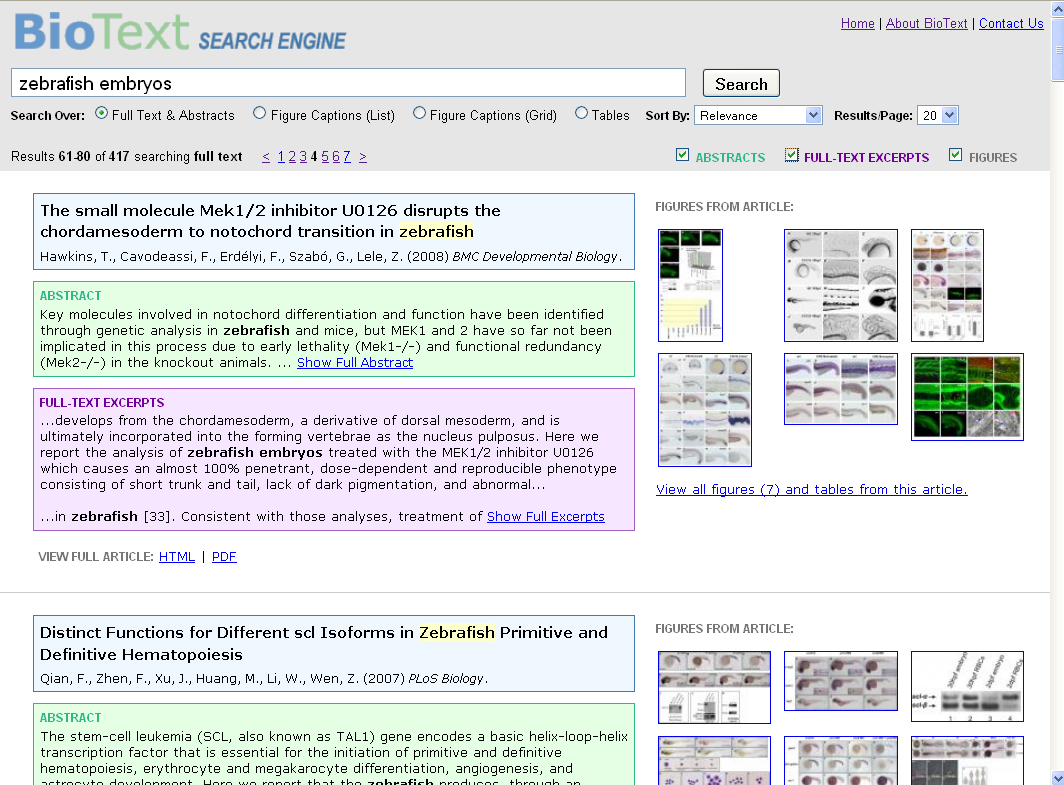
\includegraphics[width=\columnwidth]{./biotext3.png}
    \vspace{-20pt}
    \caption{Search results in the BioText system
        (\href{https://searchuserinterfaces.com/book/sui_references.html\#hearst2007bse}{Hearst et~al., 2007}),
        in which rich document surrogate information is shown, including figures extracted from the articles,
        query term highlighting and boldfacing, and an option to expand or shorten extracted document summaries.
        From \url{http://biosearch.berkeley.edu}.}
    \label{fig:figure-2}
    \vspace{-10pt}
\end{figure}

\subsection{Allow Sorting of Results by Various Criteria}

Another effective form of feedback in the display of search results allows for the dynamic sorting of
search results according to different ranking criteria (e.g., recency, relevance, author, price, etc.).
An effective interface for displaying results sortable along several dimensions at once uses a sortable
columns format, as seen in email search interfaces, some product search, and some bibliographic search
(see \autoref{fig:figure-3}). With this
view, users can sort results according to different criteria, while being able to visually compare those
criteria, because the changes are directly visible (\href{https://searchuserinterfaces.com/book/sui_references.html#reiterer2000iia}{Reiterer et~al., 2000}, \href{https://searchuserinterfaces.com/book/sui_references.html#cutrell2006fff}{ Cutrell et~al., 2006b}). This kind of view is
typically more effective than showing choices hidden behind drop-down menus. Grouping search results by
categories is also an effective form of feedback, as discussed in the section below on integrating
navigation and search.

\begin{figure}[ht]
    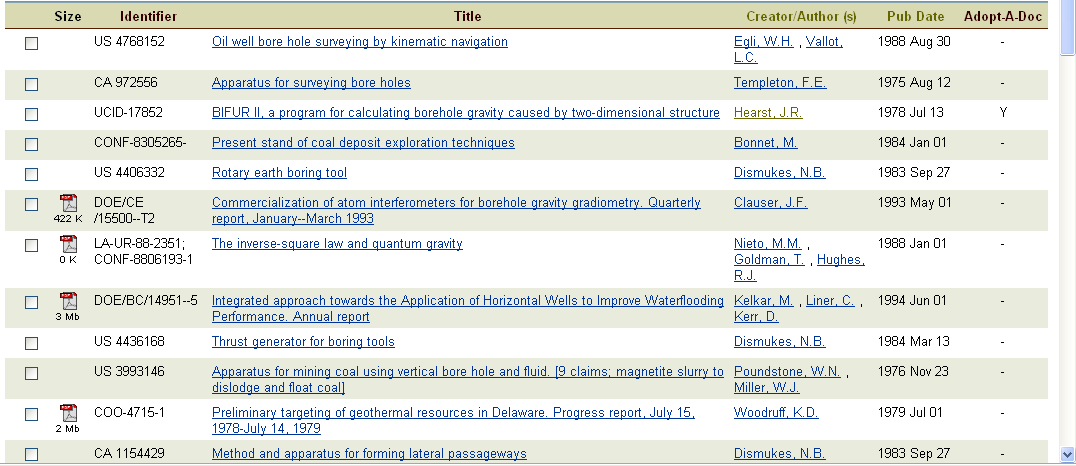
\includegraphics[width=\columnwidth]{./doecolumns.png}
    \vspace{-20pt}
    \caption{An example search results listing, on the query {\em  bore hole
    gravity}, that allows sorting results listings columns representing bibliographic fields (author,
    title, date, etc.). From the Energy Citations Database published by the U.S. Department of Energy
    (DOE) Office of Scientific and Technical Information (OSTI), \url{http://www.osti.gov/energycitations}.
    }
    \label{fig:figure-3}
    \vspace{-10pt}
\end{figure}

\subsection{Show Query Term Suggestions}

After a user has issued a query, it has been shown useful to provide feedback in the form of
automatically-generated query term suggestions and refinements. These include spelling correction
suggestions as well as suggestions of related or alternative query terms. The phrase {\em  term
expansion} is usually applied to tools that suggest alternative wordings. Usability studies are
generally positive as to the efficacy of term suggestions when users are not required to make relevance
judgements and do not have to choose among too many terms (\href{https://searchuserinterfaces.com/book/sui_references.html#bruza2000iis}{Bruza et~al., 2000}, \href{https://searchuserinterfaces.com/book/sui_references.html#anick2003utf}{ Anick, 2003}, \href{https://searchuserinterfaces.com/book/sui_references.html#white2007sup}{ White et~al., 2007}, \href{https://searchuserinterfaces.com/book/sui_references.html#divoli2008esg}{ Divoli et~al., 2008}). A study of session
logs of the Dogpile Web search engine showed found that 8.4\% of all queries were generated by the
reformulation assistant provided (\href{https://searchuserinterfaces.com/book/sui_references.html#jansen2007wsi}{Jansen et~al., 2007b}). \autoref{fig:figure-4} shows an
example of a term expansion interface provided by Yahoo.

A related recent development in rapid and effective user feedback is an interface that suggests a list
of query terms dynamically, {\em  as the user types the query}, and that match the query or are
semantically similar to it in some way. (This is sometimes referred to as {\em  incremental search}.)
For example, typing the letters {\bf  ba} on the Ask.com Web search engine shows query suggestions
including {\em  baby names, barnes and nobel, barack obama}, and {\em  bank of america}. Adding an {\bf 
n} to make a query of {\bf  ban} changes the suggestions to include {\em  banana republic,
bankruptcy}, and {\em  bangladesh}. The query suggestions are often tailored to the underlying
information collection. For example, a site that shows statistics about different airports
(flightstats.com) dynamically adjusts airport names as the user types in letters. Beginning with {\bf 
s} shows hits not only on airports whose three-letter code begins with ``s'', but also for airports
whose city name or country name begins with this letter. (These include Palma Mallorca airport in Spain,
Suvarnabhumi airport in Bangkok, and SFO in San Francisco, CA.) Adding the letter {\bf  f} eliminates
all of these except SFO, but shows less frequented airports such as Sfax El Maou airport in Tunisia.
Dynamic query term suggestions are a promising intermediate solution between requiring the user to think
of terms of interest (and how to spell them) and navigating a long list of term suggestions.

\begin{figure}[ht]
    \vspace{-5pt}
    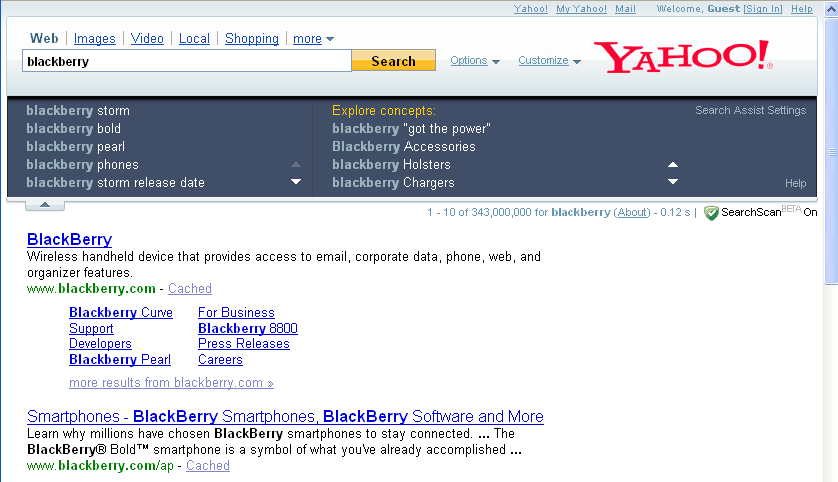
\includegraphics[width=\columnwidth]{./yahoo-search-assist.png}
    \vspace{-20pt}
    \caption{Example of an interface for showing two types of search
    assistance, from Yahoo. The left hand column shows suggestions dynamically as the user types their
    query. These suggestions usually match the prefix characters of the query. The right hand column shows
    suggestions of related terms after the query has been submitted. These need not contain characters
    from the original query. (Reproduced with permission of Yahoo! Inc. 2009 Yahoo! Inc. YAHOO! and the
    YAHOO! logo are registered trademarks of Yahoo! Inc.)}
    \label{fig:figure-4}
    \vspace{-5pt}
\end{figure}

Returning to \autoref{fig:figure-4}, this
search assistance tool uses a ``sliding tray'' that opens automatically based on heuristics corresponding
to user behavior (\href{https://searchuserinterfaces.com/book/sui_references.html#anick2008als}{Anick and Kantamneni, 2008}). For instance, if the user pauses in typing
before hitting the {\bf  Enter} key, the tray will slide out showing dynamic query suggestions. The
view shown here appears after a query has been entered, and the left hand column of suggestions in
\autoref{fig:figure-4}
shows term suggestions that are related to the query.

A log study on 100,000 visitors to the Yahoo site over 17 weeks found that this tool was heavily used,
with 30\% of those exposed to it choosing to interact with it during the first exposure, increasing to
37\% by the 17th week (\href{https://searchuserinterfaces.com/book/sui_references.html#anick2008als}{Anick and Kantamneni, 2008}). There was also a high degree of iterative
interaction with the tool. However, a small eye-tracking study showed that the interface includes a
design error that is often seen in experimental search interfaces (\href{https://searchuserinterfaces.com/book/sui_references.html#anick2008als}{Anick and Kantamneni, 2008}). In this error, the interface showed two
kinds of hints next to each other. Users are unlikely to understand the difference in meaning between
the types of suggestions in the left hand and right hand columns, because the suggestions themselves are
similar and users may not know, or need to know, the difference between dynamic suggestions and
after-query suggestions. (A smaller problem is that only one column has a visible label.) A better
design would be to show the dynamic suggestions as the query is being typed, and then replace these with
the related term suggestions after the query is entered (via hitting the return key or selecting the {\em 
Search} button). When the user resumes typing, the dynamic suggestions should replace the related
terms.

It is generally not a good idea to make people remove terms to increase relevance. For instance, \href{https://searchuserinterfaces.com/book/sui_references.html#ahn2007}{Ahn et~al., 2007} found that keyword removal caused about four times more harm
than adding keywords for building user profiles. The essence of the problem is that the space of what is
not relevant is far larger than the space of what is relevant. This is not to say that adding a ``NOT''
operator to a query is never useful, but rather that an interface should not be founded on the idea that
users will remove irrelevant terms or documents.

\subsection{Use Relevance Indicators Sparingly}

In the past it was common for search engines to show a numerical score or graphical bars or icons such
as a row of stars alongside the document surrogate to indicate the relevance score for the documents (\href{https://searchuserinterfaces.com/book/sui_references.html#shneiderman1997csu}{Shneiderman et~al., 1997}). However, these have fallen out of
favor, most likely because the meaning of the relevance score is opaque to the users (\href{https://searchuserinterfaces.com/book/sui_references.html#white2007sup}{White et~al., 2007}) , and the vertical position on the page is a strong and effective signal of the
relative relevance of the results. It should be noted that graphical indicators of other kinds of
information -- such as using a line of stars to indicate how favorably reviewed an item is -- can be
quite useful.

Innovative visualization techniques for graphically showing the distribution of the query terms within
the retrieved documents have been developed (\href{https://searchuserinterfaces.com/book/sui_references.html#hearst95b}{Hearst, 1995}, \href{https://searchuserinterfaces.com/book/sui_references.html#reiterer2005aic}{ Reiterer et~al., 2005}, \href{https://searchuserinterfaces.com/book/sui_references.html#meredith06}{ Meredith and Pieper, 2006}), but are used primarily in text
analysis interfaces rather than in standard search.

\subsection{Support Rapid Response}

For search interfaces, rapid response time is critical to support effective feedback. A perceivable lag
interrupts peoples' thought processes; rapid response allows searchers to work with ``flow.'' Providing
highly responsive interactive results is important for dynamic search results suggestions, and fast
response time for query reformulation allows the user to try multiple queries rapidly. If the system
responds with little delay, the user does not feel penalized for trying inaccurate or general queries
that are ``in the ballpark'' but not quite right. This allows the user to rapidly move closer to their
goal and learn more about their search topic with each query.

Research suggests that when rapid responses are not available, search strategies change. For instance, a
search engine for users in the developing world in which the round trip for retrieval results can be a
day or more requires accurate, thoughtful query formulation (\href{https://searchuserinterfaces.com/book/sui_references.html#thies2002sww}{Thies et~al., 2002}). It should also be noted that for some specialized search
applications in which the results are the final desired information, users are not unduly penalized by
having to wait, such as for systems that search for airline flights. These sites wisely tend to show a
graphical animation while processing the user's request, to reduce feelings of impatience.

\section{Balance User Control with Automated Actions}

\href{https://searchuserinterfaces.com/book/sui_references.html#greene2000pao}{Greene et~al., 2000} write that ``Users prefer comprehensible, predictable, and
controllable environments.'' This is a good design guideline in general. However, in the design of
technology, there is often a tradeoff between the system taking control for the user versus the user being
in control of details of the system's behavior. For example, millions of people enjoy the ease and
convenience of taking snapshots with point-and-shoot digital cameras, where there is no need to fuss with
the focus, shutter speed, or lighting because the camera automatically figures out the settings. However,
on those occasions in which the user wants to override the camera's default behavior (say, in very low
light), it can be difficult to quickly determine how to accomplish this. Similarly, in the design of
search algorithms and interfaces, there is a delicate balance between clever but opaque operations that
correctly anticipate searcher's needs most of the time and less powerful or less effective designs that
are however easily understandable and give the user control over system behavior.

Below are two important types of search interface design decisions that must consider the tradeoff between
opaque system control and transparent user control: results ordering and query transformations.

\subsection{Rank Ordering in Web Search}

The most prominent case of opacity in the operation of search interfaces is the rank ordering of
retrieval results.

As discussed above, most users have little understanding of how search technology works, and the
mechanisms behind search results ordering are especially mysterious. Early Web search engines used a
variation of vector-based statistical ranking, which is difficult to understand, in part because the
system might show a document that has many hits on a rare term higher than a document that contains a
few hits on every term in the query (\href{https://searchuserinterfaces.com/book/sui_references.html#nytimes98}{Lake, 1998}). Furthermore, Web queries
usually contain only a few words, while statistical ranking was originally designed for paragraph-length
queries.

Sometime in the late 1990's, the Hotbot search engine introduced conjunctive (AND-based) query analysis
for Web search ranking, meaning that every word in the query must be present in the document in order
for that document to be shown (\href{https://searchuserinterfaces.com/book/sui_references.html#glossbrenner1999sea}{Glossbrenner, 1999}). This behavior
is more transparent than the statistical approach because the searcher knows that every page retrieved
contains at least one instance of every word they typed. Behind the scenes, the system may give more
weight to pages in which the terms occur more frequently, but the user does not need to know that detail
in order for the retrieval strategy to be understandable. Also in the late 1990's, Google improved
conjunctive ranking by assigning higher weight to documents in which query terms co-occurred in close
proximity to one another, which had been shown by others to improve precision (\href{https://searchuserinterfaces.com/book/sui_references.html#hearst96a}{Hearst, 1996}, \href{https://searchuserinterfaces.com/book/sui_references.html#clarke96}{ Clarke et~al., 1996}), and which has the advantage of producing more
useful document summaries (\href{https://searchuserinterfaces.com/book/sui_references.html#tombros1998aqb}{Tombros and Sanderson, 1998}). Google also incorporated a ``popularity'' measure, PageRank (\href{https://searchuserinterfaces.com/book/sui_references.html#page1998pcr}{Page et~al., 1998}). The fact that
popular web pages appear higher in the results is understandable for lay users even though the algorithm
for computing popularity would not be widely understood.

Although AND-based ranking has been quite effective, today the pendulum is swinging the other way.
Sophisticated users are issuing longer queries, and the rise of natural language search engines is
encouraging longer and more complex queries. As queries get longer, it becomes necessary to relax the
constraint that all words appear in the retrieved documents, or at least to downweight their importance
in proximity to the content words. Today, a user can enter a query {\bf  typing while recovering from
clavical surgery} into Google and it successfully finds relevant documents by ignoring the role of
the syntactic structuring words {\bf  while} and {\bf  from} and returning pages in which {\bf 
recovering} occurs only in hyperlinks pointing to the page. In order for this kind of sophisticated
processing to avoid the confusing behavior of earlier statistical algorithms, the lack of transparency
must be offset by the relevance and meaningfulness of the returned results.

Perhaps the most understandable and transparent way to order search results is according to how recently
they appeared. In fact, for some information collections, such as news, chronological ordering can be
preferred over rank ordering. \href{https://searchuserinterfaces.com/book/sui_references.html#dumais2003svs}{Dumais et~al., 2003} found that users preferred chronological order over rank order when
searching over their personal information. Bioscience researchers often prefer to see scientific
articles presented according to recency. However, for web search, relevance ranking is a necessity
because time of first appearance for a Web page is of secondary importance in most cases.

\subsection{Query Transformations}

Another important issue in the tradeoff between system cleverness and user control lies with query
transformations. Some search engines make subtle changes to queries to improve results. For example,
Microsoft's web search automatically converts words like {\bf  vs.} to {\bf  versus}. The lack of user
control in this feature is mitigated by the fact that this transformation nearly always matches the
searcher's intention. As another example, Google returns pages that contain people's names for which the
middle initial is missing, even if the original query specifies the middle initial. Although a useful
feature, this could frustrate a searcher who is trying to distinguish between two people with similar
names.

A classic case of system behavior that is opaque to system users is the elimination of {\em  stopwords}
from user queries. (Stopwords are the most common words in the language, usually what linguists call
``closed-class'' words in that new ones rarely enter the language. Examples from English are articles such
as {\em  a, an, the} and prepositions such as {\em  in, on}.) In a famous example in the early days of
Web search, a searcher who typed {\bf  ``to be or not to be''} in a search engine would be shocked to be
served empty results. In 1996, a review of eight major search engines found that only AltaVista could
handle the Hamlet quote; all others ignored stopwords (\href{https://searchuserinterfaces.com/book/sui_references.html#peterson1997eis}{Peterson, 1997}, \href{https://searchuserinterfaces.com/book/sui_references.html#sherman01}{ Sherman, 2001}). (Stopword elimination is common in statistical ranking
systems for which a paragraph-length query is assumed; not indexing stopwords by position results in
significant savings in indexing time and disk space.) Today, this problem is solved on all the major Web
search engines.

The application of morphological analysis (stemming) has long yielded mixed results in the information
retrieval literature: in some cases it helps, and in others it degrades search results. From a user
expectations perspective, on the one hand, searchers express surprise if the computer is not ``smart''
enough to do simple transformations, such as automatically converting {\bf  woman's rights} in the
query to match {\bf  women's rights} in documents (\href{https://searchuserinterfaces.com/book/sui_references.html#twidale1998dis}{Twidale and Nichols, 1998}). But on the other
hand, if morphological analysis is done too aggressively, the meaning of the query can be distorted. For
example, Google converts the word {\bf  typing} to {\bf  type} in the query {\bf  typing after clavicle
surgery}, which yields some results that do not discuss the act of typing. These effects are mild
so long as the stemming is applied lightly, and a mix of the word forms is allowed to contribute to the
results. But if the system consistently overrules the user's intention, the user may become justifiably
frustrated.

In the case of automatic spelling suggestions, the system should offer the choice to the user without
forcing an acceptance of an alternative spelling, in case the system's correction does not match the
user's intent. But on the other hand, if the user makes a blatantly incorrect typographical error, it
can be annoying to see only irrelevant results, and the system may return low-quality Web pages. To
balance this tradeoff, when encountering what the system believes is an erroneously spelled query term,
many Web search engines show some hits that contain words that they guess are the correct spelling
interwoven with other hits that contain the purportedly incorrect spelling.

\section{Reduce Short-Term Memory Load}

The interface guideline ``reduce the user's memory load'' is very important for information-rich system
interfaces. The main idea behind this heuristic is to show users relevant information rather than require
them to remember or keep track of it. Several methods applicable to search interfaces are described in the
subsections below.

\begin{figure}[ht]
    \vspace{-5pt}
    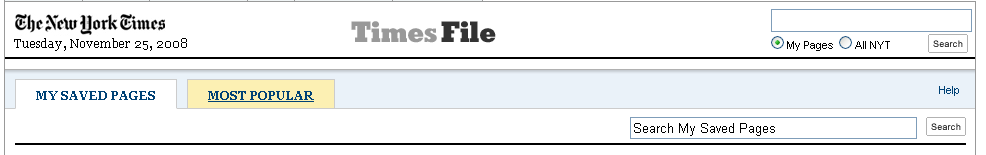
\includegraphics[width=\columnwidth]{./nytimes-searchbox.png}
    \vspace{-20pt}
    \caption{Example of a query form that provides a reminder of which set of
    content is being searched over, from {\em  The New York Times}.}
    \label{fig:figure-5}
    \vspace{-5pt}
\end{figure}

\subsection{Suggest the Search Action in the Entry Form}

A useful interface trope that has arisen recently is, rather than showing a blank entry form, the
designer places text within the entry form to indicate what action will result from using that form.
This text is usually shown in grayed-out font, to signal that it is intended to be replaced by the
user's text. (The text within the form disappears when the user clicks in the form.) This is especially
useful in search interfaces as a way to indicate that the user would be searching over an alternative
collection, or when attempting to provide a ``search within these results'' feature. The lower right hand
corner of \autoref{fig:figure-5} shows an
example from the Web site of {\em  The New York Times}, that makes it clear that a query in that entry
form searches over the user's saved pages, as opposed to searching over the site as a whole. This design
works in part because the user must look at the text in the entry form in order to select the form and
begin typing; it demands the user's attention, but is not distracting because it provides the
information exactly at the point in the user's workflow that it is needed at.

In the upper right hand corner is shown a more standard approach to allowing users to choose between
collections. It shows a search box with a radio button that selects which collection to search over.
Most studies suggest that users do not notice or change the choices in this type of interface, in part
because they do not notice the option while they are entering their query. A radio button or other
choice selector, such as a drop-down menu, is more likely to be noticed after the query is issued when
retrieval results are being viewed. Thus, selectors for sorting the search results (by date, by price,
etc.) after the query are used with some frequency.

\subsection{Support Simple History Mechanisms}

Research shows that people are highly likely to revisit information they have viewed in the past and to
re-issue queries that they have written in the past (\href{https://searchuserinterfaces.com/book/sui_references.html#jones2002oft}{Jones et~al., 2002}, \href{https://searchuserinterfaces.com/book/sui_references.html#milicfrayling2004ssu}{ Milic-Frayling et~al., 2004}). In one large study, 40\% of
people's search results clicks were on pages that they had clicked on before over the course of a year,
with 71\% of these using the identical query string as before (\href{https://searchuserinterfaces.com/book/sui_references.html#teevan2006hri}{Teevan et~al., 2006a}). In a survey associated with this study, 17\% of interviewees reported
``not being able to return to a page I once visited'' as one of the ``biggest problems in using the web.''
Therefore, allowing search over recently viewed information can improve a user's productivity (\href{https://searchuserinterfaces.com/book/sui_references.html#dumais2003svs}{Dumais et~al., 2003}). Web browsers, as opposed to search engines, can provide much of this
functionality. For example, the Chrome Web browser supports information revisiting by showing a grid of
thumbnail images representing a user's most frequently visited web pages, and the drop-down menu from
the many browser Web address bars shows recently visited pages. Search engines themselves can provide
query history, as well as history of previously selected pages if the user agrees to having that
information recorded. The PubMed bioscience journal service shows recently issued queries and visited
documents in a simple history display (see \autoref{fig:figure-6}).
Similarly, many shopping Web site show recently viewed items in a graphical form. Thumbnail images have
also been experimented with in search results listing, both for reminding searchers of previously
visited pages and for suggesting information about the hit, such as its genre.

\begin{figure}[ht]
    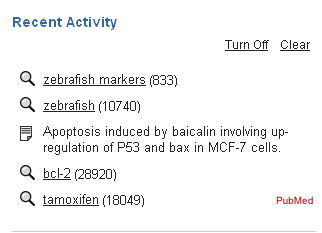
\includegraphics[width=\columnwidth]{./pubmed-recentactivity.png}
    \vspace{-20pt}
    \caption{The PubMed interface, published by the U.S. National Library of
    Medicine, for showing recent queries and recently accessed documents in a simple history display.}
    \label{fig:figure-6}
\end{figure}

In Web sites that integrate category selection with search, a history mechanism called {\em 
breadcrumbs} is used for keeping track of the sequence of navigation operations that the user has
taken to arrive at the current view of objects (discussed in more detail below).

\subsection{Integrate Navigation and Search}

A well-established principle of human memory is that it is often easier to recognize a word or name than
it is to think up that word. Thus in many situations it is useful to prompt the searcher with
information related to their information need. Browsable information structures, such as links on a Web
site or a table of contents for a book, give an overview of the contents of a collection, allowing the
searcher to navigate to the information of interest by following links or narrowing by selecting
categories. Information structures can also impose an organization on the results of search. To be fully
effective, navigation interfaces should allow the user to interleave keyword queries within existing
information structures, smoothly integrating navigation with search. This means that after a keyword
search, results should be organized into the navigation structure, and that after navigation steps,
keyword search should be available over the current subset of information items.

In search interfaces, category systems are the main tool for navigating information structures and
organizing search results. A category system is a set of meaningful labels organized in such a way as to
reflect the concepts relevant to a domain. In search interfaces, categories are typically used either
for selecting a subset of documents out from the rest, thus narrowing the results, or for grouping
documents, dividing them into (potentially overlapping) subsets, but keeping the documents visible. They
can also be used for ordering and sorting search results.

Category system structure in search interfaces is usually one of {\em  flat}, {\em  hierarchical}, or
{\em  faceted}. A flat list of categories works well for presenting a list of choices with which to
narrow the contents of a collection, but needs to be limited to a small set in order to be scannable.
Hierarchical (or tree-structured) category systems are useful and can be easy to understand for
relatively simple information structures. However, a problem with assigning documents to single
categories within a hierarchy is that many information items are best described by multiple different
categories simultaneously.

This use of {\em  hierarchical faceted metadata} provides a usable method for allowing users to browse
information collections according to multiple categories simultaneously (\href{https://searchuserinterfaces.com/book/sui_references.html#hearst2000ngw}{Hearst, 2000}, \href{https://searchuserinterfaces.com/book/sui_references.html#hearst02}{ Hearst et~al., 2002}). The main idea is
to build a set of category hierarchies, each of which corresponds to a different facet (dimension or
feature type) that is relevant to the collection to be navigated. Each facet has a set of labels
associated with it, and if this set is large, it may be organized into a hierarchy. After the facet
hierarchies are designed, each item in the collection can be assigned any number of labels from any
number of facets. In a properly designed faceted navigation interface, the user can browse the
information collection from any of the different facets as a starting point, and after starting with one
facet, can then navigate using any other facet. Usability results suggest that this kind of interface is
highly usable for navigation of information collections with somewhat homogeneous content (\href{https://searchuserinterfaces.com/book/sui_references.html#flamenco01}{English et~al., 2001}, \href{https://searchuserinterfaces.com/book/sui_references.html#hearst02}{ Hearst et~al., 2002}, \href{https://searchuserinterfaces.com/book/sui_references.html#yee03}{ Yee et~al., 2003}).

This kind of interface is heavily used on Web sites today, including shopping and specialized product
sites, restaurant guides, and online library catalogs. \autoref{fig:figure-7} shows an
example in which a user interested in finding local events to attend on zvents.com can select a city in
which the event is to take place ({\em  Berkeley}) and then select a type of event ({\em  Community})
in this case. The faceted display allows the user to select the order in which to choose the categories,
and the search results are narrowed accordingly to show only those events that will take place in
Berkeley and have to do with community. Beneath each facet category label are shown the subcategory
labels along with {\em  query previews} (\href{https://searchuserinterfaces.com/book/sui_references.html#plaisant99}{Plaisant et~al., 1999}) showing how many documents are associated with each category. For instance,
one can see how many of the 43 community events taking place in Berkeley take will be held each of the
different neighborhoods, and one can see how many of each type of event is available ({\em  Activism,
Health, Science}, etc.). Note also the use of light-colored text within the query boxes to indicate
which kind of information should be entered into each query box.

\begin{figure}[ht]
    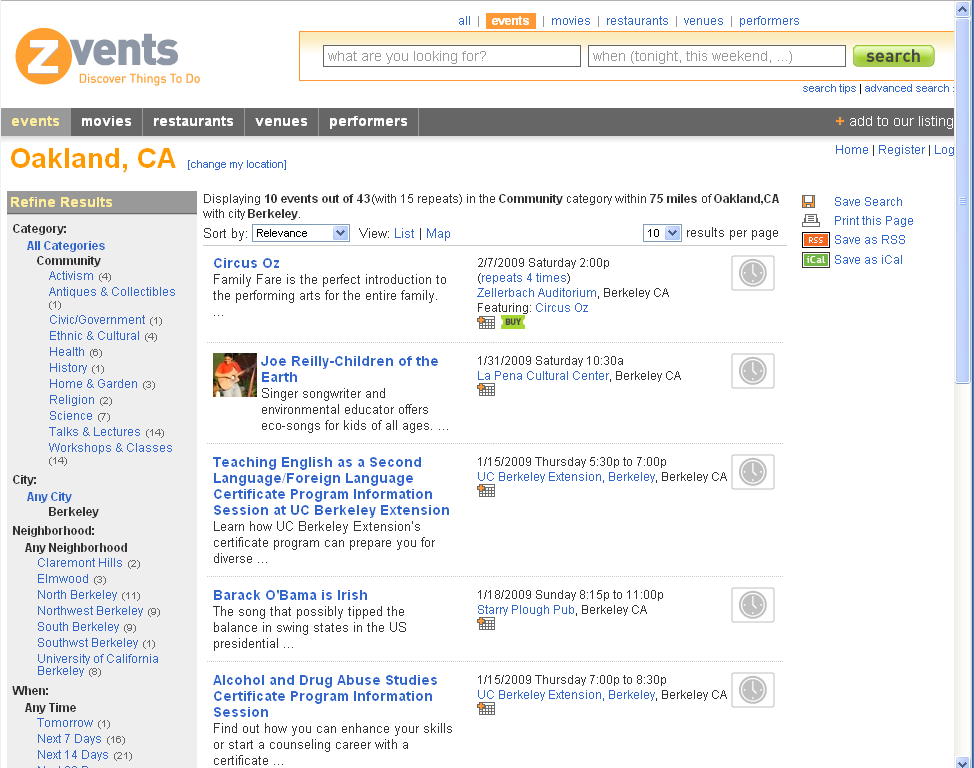
\includegraphics[width=\columnwidth]{./zvents.png}
    \vspace{-20pt}
    \caption{Faceted navigation interface for the zvents.com local events
    web site. The user has selected the city of ``Berkeley'' from the {\em  Location} facet and ``Community''
    from the event {\em  Category} facet, and each of these selections can be further refined (by
    ``Neighborhood'' for {\em  Location} or by type of community activity). Beside each narrowing category
    is shown in parentheses how many items will result from selecting that category. Or the user can opt
    to narrow by another faceted entirely, such as {\em  When}.}
    \label{fig:figure-7}
    \vspace{-10pt}
\end{figure}

\section{Provide Shortcuts}

The ``provide shortcuts'' guideline usually refers to providing alternative interface mechanisms for
practiced users of an interface. The classic example is keyboard shortcuts for menu items that otherwise
require pulling down and selecting from menus. Keyboard shortcuts can save time and effort when the user
is typing, as the shortcuts remove the need to move hands away from the keyboard to the mouse. But there
is a barrier to using shortcuts, as they require memorization.

An alternative way to think about shortcuts, which is more applicable to search interfaces, is to provide
targeted hints about where to go next. For example, certain variations on the document surrogate appear to
be successful in practice. One technique that appears to be especially useful for Web search is what are
known as {\em  sitelinks} or {\em  deep links}. In this view, in the search results, beneath the
top-positioned hit, is shown an indented list of important pages from that hit on its Web site, along with
a link to more pages from that web site. Presumably the links are chosen because they represent
frequently-visited pages within the site, thus saving the user a step or two by allowing them to navigate
directly to a page of interest from the search results page. For example, in \autoref{fig:figure-4}, for a query
on {\bf  blackberry}, the top hit is the home page of a maker of mobile devices, {\em 
www.blackberry.com}. Beneath the link for this hit are shown links to important pages within the site
such as {\em  Support} and {\em  Developers} as well as to pages for popular products such as {\em 
Blackberry Curve}. In Google's implementation of this idea, another kind of shortcut is sometimes
provided: a search form is shown beneath the hit which allows the user to search within that domain
directly from the search results page.

As another kind of shortcut, for certain well-defined and predictable information needs, major Web search
engines today attempt to ``guess'' the information need from a very terse query based on what kinds of
information have been found to be valuable to searchers on that type of query in the past. The relevant
``answer'' corresponding to that information need is shown directly in the search results page. For example,
Yahoo search will display a ``shortcut'' showing the current local time in Kathmandu, Nepal, for any of the
following queries: {\bf  time kathmandu}, {\bf  kathmandu current time}, and {\bf  what time is it?
katmandu}. In Google, at one time a query on {\bf  rentals seattle} returned a special form directly
in the results list that allowed the user to specify details of a housing search. All Web search engines
show links to shopping sites and review sites in response to purchase-oriented queries (such as {\bf 
digital cameras}) and images in response to queries for which images are likely to be evocative (such
as {\bf  sunsets}). In a sense, this kind of intention prediction is a form of shortcut, eliminating the
need for the user to know precisely how to specify a command, and also reducing the need to navigate to
external Web pages to find the desired information.

\section{Reduce Errors}

The steps taken by interface designers to reduce the likelihood of user errors tend to overlap with other
guidelines. One key example discussed above is to provide accurate suggestions for typographic and
spelling errors. Some additional heuristics are described below.

\subsection{Avoid Empty Results Sets}

A general rule of thumb for search usability is to avoid showing the user empty results sets. Spelling
correction and term expansion can help with this. Another mechanism mentioned above is to use query
previews to show how many documents will result if a particular navigation step is taken. Interfaces
that allow users to select many different attributes from different categories simultaneously (e.g., for
a recipes interface, selecting {\em  dessert} and {\em  low-fat} and {\em  cheese}) may run the risk
of turning up empty results. A faceted interface with query previews would show the user that after
selecting {\em  dessert} and {\em  low-fat}, the list of ingredients has zero hits on {\em  cheese},
so the user would know they have to relax one of the already chosen constraints to get non-empty
results.

\subsection{Address the Vocabulary Problem}

Another form of error can come from using wording that the user does not recognize in navigational cues
or in menu items, or in the search itself. A general problem with searching via keyword matching lies
with the ``productivity of language'' -- also known as ``the vocabulary problem'' -- that the same idea can
be expressed in an astonishing variety of ways. Consider, for example, the different ways one might ask
the price of a camera in English:

\begin{itemize}
\item How much does that camera cost? 
\item How much for that camera? 
\item That camera. How much? 
\item What is the price of that camera? 
\item Please price that camera for me. 
\item What're you asking for that camera? 
\item How much will that camera set me back? 
\item What are these cameras going for? 
\item What's that camera worth to you? 
\end{itemize}

To prove scientifically how word choice varies among people, \href{https://searchuserinterfaces.com/book/sui_references.html#furnas1987vph}{Furnas et~al., 1987} explored the
vocabulary variation phenomenon by studying spontaneous word choice for five different computer
application domains. These included asking 48 typists to describe 25 text editing markup operations, and
asking 337 college students to describe a set of 50 common objects. The experimenters counted how often
each word or phrase was used to label each operation or object, and looked at the agreement between
people.

The probability that two typists would suggest the same word to describe a markup operation was .11, and
the probability that two college students would name an object with the same word was .12. \href{https://searchuserinterfaces.com/book/sui_references.html#furnas1987vph}{Furnas et~al., 1987} then measured the
effect of choosing the most commonly selected word for each concept, and comparing this to the terms
people originally selected. This increases the probability of agreement to .22 for the markup operations
task and .28 for the common objects naming task. When they broadened the vocabulary to include the three
most frequently elicited terms for each concept (simulating, in a sense, a thesaurus), they found the
probability of agreement increased to .49 for the markup task and .48 for the object naming task.
Further analysis indicated that even with 15 aliases per term, only 60-80\% of the original terms people
thought of would be matched.

The fact that different people express similar concepts in different ways has deep implications for the
design of information systems. It suggests that a searcher might not use the same combinations of terms
that the authors of the most relevant documents used. Term expansions have been shown to be an effective
way to help with this problem. It also suggests that terminology for labeling interface elements must be
chosen very carefully. In fact, terminology choice is so important that a design technique has been
developed, called {\em  card sorting}, whose goal is to attempt to converge on the most reliable,
predictable categories and labels for a given information structure (\href{https://searchuserinterfaces.com/book/sui_references.html#kuniavsky2003oue}{Kuniavsky, 2003}).

\section{Recognize the Importance of Small Details}

Search interfaces must show rich and complex information, and small details can make the difference
between a successful and a failed design. There is ample evidence that details in a search interface can
deeply affect how the information seeker executes their search.

For example, \href{https://searchuserinterfaces.com/book/sui_references.html#franzen2000vai}{Franzen and Karlgren, 2000} found that showing study participants a
wider entry form encouraged them to type longer queries. \href{https://searchuserinterfaces.com/book/sui_references.html#allen1994psl}{Allen, 1994} showed that varying the order in which document surrogate information was shown to
searchers dramatically effected how much searchers learned about the information (in this case, subject
headings) available in a document collection. \href{https://searchuserinterfaces.com/book/sui_references.html#russell:bll}{Russell et~al., 2006} experimented with a visualization that
showed documents as clusters of icons in a two-dimensional space, and concluded that this view reduced
performance because the representation did not match human perceptual capabilities well. Several
researchers have shown that users of Web search engines expect the first few results returned to be more
relevant than those that follow, and are more likely to click on the first two hits than they should be
when the results ordering is reversed (\href{https://searchuserinterfaces.com/book/sui_references.html#joachims2005aic}{Joachims et~al., 2005}).

As another example of the influence of small design decisions on user experience, in an early version of
the Google spelling suggestions interface, searchers generally did not notice the suggestion at the top of
the page of results. In the initial design, the interface showed a suggestion sentence worded as follows:
``If you didn't find what you were looking for ...'' At the same time, Google was receiving feedback from
searchers complaining that they were getting incorrect results for their queries. According to a product
VP at Google (\href{https://searchuserinterfaces.com/book/sui_references.html#hurst02}{Hurst, 2002}, \href{https://searchuserinterfaces.com/book/sui_references.html#sinha05}{ Sinha, 2005}),
in many of these cases, the spelling suggestions module had suggested an appropriate correction, but
searchers did not notice the information at the top of the page. Instead, they focused on the search
results, scrolling down to the bottom of the page scanning for a relevant result but seeing only the very
poor matches to the misspelled words. They would then give up and complain that the engine did not return
relevant results. To improve the likelihood of searchers noticing the spelling suggestions, two small
interface adjustments were made. The first was to repeat the spelling suggestion at the bottom of the
page. The second was to test and then shorten the wording surrounding the suggestion. On the top of the
page it now reads: {\em  Did you mean: ...} and at the bottom of the results, {\em  Did you mean to search
for: ...} with an underlined hyperlink to the results for the correctly spelled words (\href{https://searchuserinterfaces.com/book/sui_references.html#hurst02}{Hurst, 2002}, \href{https://searchuserinterfaces.com/book/sui_references.html#sinha05}{ Sinha, 2005}).

\section{Recognize the Importance of Aesthetics in Design}

A search interface designer must balance the choices of layout, placement and amount of blank space (often
referred to as ``white space''), color, contrasts among fonts' style, weight, and size. The importance of
the application of graphic design principles is established in the HCI literature. For example, \href{https://searchuserinterfaces.com/book/sui_references.html#parush10elg}{Parush et~al., 1998} performed a study comparing 16 different versions of display layout, where they
deliberately varied the quality of each design according to the graphic design principles of grouping,
density, alignment, and size. In a study with 75 participants, they found that the task time for the worst
layout was twice that of the best, and that overall, the very well designed screens resulted in shorter
search times and higher subjective preferences.

Aesthetic impressions also play an important role in user acceptance and have been found to correlate with
perceptions of an interface's quality, user satisfaction, and overall impression of a site (\href{https://searchuserinterfaces.com/book/sui_references.html#hassenzahl2004ibg}{Hassenzahl, 2004}, \href{https://searchuserinterfaces.com/book/sui_references.html#lindgaard2003ebw}{ Lindgaard and Dudek, 2003}). \href{https://searchuserinterfaces.com/book/sui_references.html#nakaradakordic2005epa}{Nakarada-Kordic and Lobb, 2005} report that viewers persevere longer in a search task on Web sites
whose design appeals to them. \href{https://searchuserinterfaces.com/book/sui_references.html#vanderheijden2003fiu}{van~der Heijden, 2003} found that the
visual appeal of a Web site affected participants' enjoyment and perception of ease of use, and to a small
degree, the usability of the system. \href{https://searchuserinterfaces.com/book/sui_references.html#norman2004edw}{Norman, 2004} also writes about the importance of aesthetics in perceived and real usability. In
the study of \href{https://searchuserinterfaces.com/book/sui_references.html#parush10elg}{Parush et~al., 1998} mentioned above, usability and aesthetic design are often intertwined, but \href{https://searchuserinterfaces.com/book/sui_references.html#benbassat2006eas}{Ben-Bassat et~al., 2006} were able to show that more aesthetic designs were perceived
as more useful even when they were slightly less useful than a comparable, less attractive design.

As an example of these effects on search interfaces, in a comparative study, \href{https://searchuserinterfaces.com/book/sui_references.html#hotchkiss07}{Hotchkiss, 2007b} asked Yahoo and MSN search users to do a query
using Google's Web search. They found that by almost every metric (including percentage of page scanned
before choosing a link, time to choose a link, and relevance of the selected link), the participants had a
better user experience on Google than using their standard search engine. \href{https://searchuserinterfaces.com/book/sui_references.html#hotchkiss07}{Hotchkiss, 2007b} attributed this difference {\em  not} to the
quality of the search results, but rather to several design choices. He noted that details in the way the
information was presented made it easier to determine relevancy, and suggested that this might be a
combination of methods of revealing information ``scent'' (most likely by showing more descriptive document
summaries that are relevant to the queries), along with subtle graphic design details. In an interview (\href{https://searchuserinterfaces.com/book/sui_references.html#hotchkiss07}{Hotchkiss, 2007b}) , a Google VP confirmed that the Web page design
is the result of careful usability testing of small design elements; for example, putting a line along the
side of a textual advertisement within the search results page, as opposed to boxing the ad in, better
integrates the ad with what people read. The Google designers pay careful attention to the aesthetic
effects of, for example, the height and width proportions for icons. \href{https://searchuserinterfaces.com/book/sui_references.html#hotchkiss07}{Hotchkiss, 2007b} also noted that Google is careful to ensure that
all information in the Web page's ``sweet spot'' (the upper left hand corner that is known to be where users
tend to look first for search results), including the ads, is of high relevance to the query. He suggested
that even if the result hits for other search engines are equivalent in quality to Google's, they
sometimes show ads that are not relevant at the top of the results list, thus degrading the user
experience.

\section{Conclusions}

This chapter has introduced the ideas and practices surrounding user interface design in general, and
search interface design in particular. It has explained some of the difficulties with search interface
design and provided a set of design guidelines tailored specifically to search user interfaces. These
guidelines include:

\begin{itemize}
\item Offer efficient and informative feedback, 
\item Balance user control with automated actions, 
\item Reduce short-term memory load, 
\item Provide shortcuts, 
\item Reduce errors, 
\item Recognize the importance of small details, and 
\item Recognize the importance of aesthetics. 
\end{itemize}

This chapter has also summarized some of the most successful design ideas that are commonly in use in
search interfaces today. This summary is based on generalizing over the results of years of research,
experimentation, and tests in the marketplace. The coming years should reveal additional new, exciting
ideas that will become reliable standards for search user interfaces.

\end{document}
\endinput